\chapter[Modélisation]{Modélisation}
\label{Modelisation}

\chapterabstract
{
Au cours de ce chapitre, la phase de développement informatique effectué pendant cette étude, ainsi que les phases de conception et de développement des modèles de prédiction grâce au Datamining dans les différentes plateformes seront présentées. Notamment, nous expliquerons en détails les grandes étapes d'installation et de configuration des outils Datamining, ensuite nous allons développer un modèle pour chaque algorithme avec les paramètres choisis par défauts pour chaque plateforme, puis nous chercherons le meilleur modèle après optimisation des hyperparamètres de ces algorithmes.
}
\pagestyle{plain}

\section{Développement informatique}\label{conf_plat}
Avant d'entamer la phase de développement des modèles de prédiction sélectionnés pour ce travail (RF, GBM, XGB et Deep learning). L'installation et la configuration des différents plateformes open source utilisées dans cette étude (\textit{WEKA}, \textit{H2O}, \textit{Scikit-learn}, \textit{Tensorflow} et \textit{Keras}) m'a exigé une période assez importante. Bien évidemment, cette phase a consisté à comprendre et à se familiariser avec le mode de fonctionnement et d’implémentation de chaque plateforme, ainsi que les librairies Datamining y incluses. En effet, cette phase m'a permis d'approfondir mes connaissances dans le domaine du  Datamining.\\

Il est à noter que toutes ces plateformes, packages et bibliothèques sont installés et configurés sur un ordinateur portable HP avec 12 Gb en RAM \footnote { Random Access Memory} et un processeur Intel\textregistered core\texttrademark i7 – 2620M CPU @ 2.70 GHz (4CPUs) $\thicksim$ 2.7 GHz. Cet ordinateur a un système d'exploitation Windows 10 (version 1803) (Cf. Fig. \ref{pc_config}). Ainsi l'installation de ces outils est établie avec des versions stable à la date de mars 2019.\\

\begin{figure}[!htb]
        \center{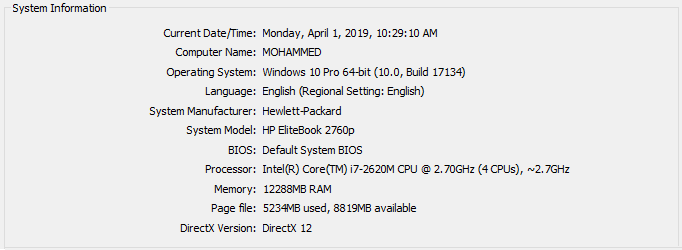
\includegraphics[width=\textwidth]{img/config.png}}
        \caption{\label{fig:my-label} Configuration de l'ordinateur utilisé pour ce travail}
        \label{pc_config}
\end{figure}


Dans la suite, les étapes de l'installation et la configuration de chaque outil Datamining sont explicitées:\\


Tout d'abord, nous avons installé la version stable 3.8 (13 février 2019) du logiciel \textit{WEKA} (Cf. Section \ref{defWeka}) qu'on a téléchargé depuis le site web officiel de l'application (www.cs.waikato.ac.nz). Ce qui a nécessité d'installer la version adaptée à Windows 10 ainsi la machine virtuelle Java VM 1.8. Une fois l'installation est terminée, nous avons augmenté l'espace mémoire allouée à Weka (heap size) de 256M par défaut à 4096M ‬pour qu'il prenne en charge les données de grande taille et d'éviter les problème de saturation de la mémoire au cours de l'exécution les phases d'apprentissage.\\

Pour la deuxième plateforme \textit{H2O} (Cf. Section \ref{defH2O}), l'algorithme \textit{XGBoost} n'a pas fonctionné pas sous H2O en Windows, donc on était obligé d’installer la plateforme H2O sous Linux.  Dans notre étude, l'installation a été effectuée sous une machine virtuelle de Linux. Cette tâche a été effectuée sous Linux Ubuntu 16.04 dans VMware Workstation avec la configuration suivante : 8GB en RAM, 2 processeurs et 30GB comme espace physique.
Une fois installé, nous avons téléchargé le fichier h2o-3.22.1.6.zip « dernière version stable à la date du 28/03/2019 » depuis le site web officiel de la plateforme (https://www.h2o.ai/).\\

Puisque \textit{H2O} se base principalement sur Java, nous avons installé openJDK 1.8. Avec la commande suivante nous pouvons lancer \textit{H2O} :
\begin{figure}[!htb]
        \center{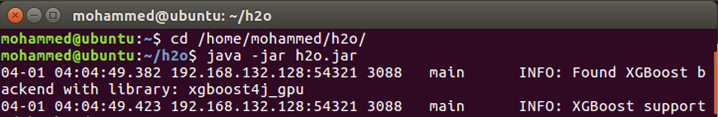
\includegraphics[width=\textwidth]{img/lanceh2o.png}}
\end{figure}

A l'issue de cette étape, nous avons le droit d’utiliser \textit{H2O} en mode web (FLOW) dans le système Windows « il suffit de taper l’adresse + port dans le navigateur (198.168.132.128 :54321 dans notre cas) ». Et pour pouvoir utiliser Python ou R, il suffit d’installer le même package \textit{h2o} (c’est-à-dire 3.22.1.6). Au cours de ce stage, nous avons opté pour le langage R. \\

\begin{wrapfigure}{r}{0.2\textwidth}
    
\includegraphics[width=0.2\textwidth]{img/condalogo.png}
\end{wrapfigure}
Pour les trois derniers outils ils ont basé principalement sur Python, alors nous avons travaillé avec Anaconda Navigateur\footnote{C'est une distribution libre et open source des langages de programmation Python et R appliqué au développement d'applications dédiées à la science des données et à l'apprentissage automatique, adaptés pour Windows, Linux et MacOS.} 3.7.1 avec une version de Python 3.7 pour \textit{Scikit-learn} et 3.6 pour \textit{Tensorflow} et \textit{Keras}.\\

Une phase préliminaire a consisté en l'installation des packages \textit{numpy} et \textit{scipy} qui sont des paquets requis pour installer \textit{Scikit-learn} ( C'est déjà expliqué dans la section \ref{defscikit}). Le moyen le plus simple d’installer \textit{Scikit-learn} consiste à utiliser \textbf{pip}\footnote{
Pip est un acronyme récursif pouvant signifier "Pip Installe des packages" ou "Pip Installe Python", c'est un outil de gestion des packages de distribution en Python} donc une fois l’installation d’Annoconda est terminé nous avons installé notre paquet \textit{Scikit-learn} en utilisant l’invite de commande annaconda comme ci-dessous:
\begin{tcolorbox}
\normalsize pip install -U scikit-learn
\end{tcolorbox}	
Ou en utilisant la command \textbf{conda} :
\begin{tcolorbox}
\normalsize conda install scikit-learn
\end{tcolorbox}	
Sous l’environnement par défaut de la distribution Anaconda. \\

Concernant \textit{Tensorflow} (Cf. Section \ref{defTensor}) et \textit{Keras} (Cf. Section \ref{defKeras}), nous étions obligé de créer un nouvel environnement Anaconda, puis l'activer pour installer les packages \textit{Tensorflow} et \textit{Keras} qui nécessite la version Python 3.6. Les étapes d'installation sont expliqués ci-dessous: \\

\begin{enumerate}
\item La création d'un environnement conda nommé « tensorflow » (vous pouvez changer le nom) en appelant la commande suivante :
\begin{tcolorbox}
\normalsize conda create -n tensorflow pip python=3.6
\end{tcolorbox}	
\item L'activation de l'environnement Conda en exécutant la commande suivante :\\
\begin{tcolorbox}
\normalsize activate tensorflow
\end{tcolorbox}	
\end{enumerate}
Une fois cette configuration est terminée, nous somme prêt à installer les bibliothèques Python utilisées pour \textit{Deep Learning}, notamment : \textit{TensorFlow} et \textit{Keras}.\\

Pour installer \textit{TensorFlow}, taper la commande suivante :
\begin{tcolorbox}
\normalsize pip install tensorflow
\end{tcolorbox}


Finalement pour installer la dernière API \textit{Keras}, on vérifie tout d'abord la présence de l’un de ses moteurs : \textit{TensorFlow}, \textit{Theano} ou \textit{CNTK}. 
il suffit de taper la commande suivante:\\
\begin{tcolorbox}
\normalsize pip install keras
\end{tcolorbox}




%%%%%%%%%%%%%%%%%%%%%%%%%%%%%%%%%%%%%%%%%%%%%%%%%%%%%%%%%%%%%%%%%%%%%%%%%%%%%%%%%%%%%%%%%%%%%%%%%%%%%%%%%%%%%%%%%%%%%%%%%%%%%%%%
\section{Développement des modèles de prédiction}
Au cours de notre étude, nous avons utilisé les méthodes du Datamining de famille d’estimateurs suivants: \textit{Random Forest} (RF), \textit{ Gradient Boosting Machine} (GBM) et \textit{eXtreme Gradient Boosting} (XGBoost), ainsi que \textit{Deep learning}. La théorie de ces algorithmes est explicitée succinctement dans la section \ref{algo_used}.\\

Pour mener à terme cette phase de modélisation, les étapes suivies pour développer chaque algorithme étaient comme suit :
\begin{enumerate}
    \item Importation des deux fichiers de données (donnée d'apprentissage et de test);
    \item Spécification des variables indépendantes (X\_train et X\_test)  et dépendant (y\_train et y\_test);
    \item Génération du modèle de prévision à partir des sorties du modèles de prévision numérique du temps AROME pour chaque algorithme par plateforme à la base des données d'apprentissage : dans un premier temps en utilisant les paramètres par défaut, ensuite en utilisant les hyperparamètres issus des méthodes d'optimisation décrites en section \ref{opt_algo};
    \item Évaluation de la performance du modèle développé en utilisant les données de test pour calculer les indices de diagnostic expliqués dans la section \ref{dig_algo_perf}.\\
\end{enumerate}

Il est à noter que pour le développement du modèle à la base de \textit{Deep learning} a nécessité la normalisation de données.\\

Dans ce qui suit, nous allons expliciter les fourchettes des hyperparamètres qu'on a utilisé au cours de ce stage pour leur optimisation afin d'obtenir le modèle par algorithme et par plateforme.\\
%%%%%%%%%%%%%%%%%%%%%%%%%%%%%%%%%%%%%%%%%%%%%%%%%%%%%%%%%%%%%%%%%%%%%%%%%%%%%%%%%%%%%%%%%%%%%%%%%%%%%%%%%%%%%%%%%%%%%%%%%%%%

\subsection*{Les hyperparamètres avec Random Search et Grid Search}\label{hyper_param}

Le réglage des hyperparamètres est une étape nécessaire lors la phase de modélisation en Machine learning. Elle permet de tester différentes configurations d'hyperparamètres pendant l'entraînement du modèle. Ces réglages peuvent fournir au développeur des valeurs optimisées pour les hyperparamètres, ce qui permet d'améliorer la précision des prédictions du modèle.\\

L'application d'entraînement gère trois catégories de données pendant l'entraînement du modèle à développer :

\begin{itemize}

\item[\ding{224}]    \textit{Les données d'entrée} (également appelées données d'entraînement) sont un ensemble d'enregistrements individuels (instances) contenant les caractéristiques importantes de la problématique de machine learning. Ces données sont utilisées pendant l'entraînement pour configurer le modèle afin qu'il puisse réaliser des prédictions précises à partir de nouvelles instances de données similaires. \\

\item[\ding{224}]   \textit{Les paramètres} du modèle sont les variables que la technique de machine learning sélectionnée utilise pour s'adapter aux données. Par exemple, un réseau de neurones profond (Deep Neural Network ou DNN) est composé de nœuds de traitement (neurones). Chacun d'entre eux effectue une opération spécifique sur les données lors de leur propagation à travers le réseau. Lorsque le DNN est entraîné, chaque nœud possède une valeur de pondération qui indique au modèle l'impact de ce nœud sur la prédiction finale. Ces pondérations sont un exemple de paramètres associés au modèle. \\

\item[\ding{224}]     \textit{Les hyperparamètres} sont les variables qui régissent le processus d'entraînement lui-même. Par exemple, une partie de la configuration d'un réseau de neurones profond consiste à décider combien de couches de nœuds cachées seront utilisées entre la couche d'entrée et la couche de sortie, ainsi que le nombre de nœuds que chaque couche doit utiliser. Ces variables ne sont pas directement liées aux données d'entraînement. Ce sont des variables de configuration. Notez que les paramètres changent au cours d'une tâche d'entraînement, alors que les hyperparamètres sont généralement constants pendant une tâche.\\
\end{itemize}

Dans ce qui suit, nous résumons dans des tableaux les fourchettes utilisées pour l'optimisation des hyperparamètres pour les plateformes \textit{Scikit-learn} et \textit{H2O} à la base deux méthodes : Grid-Search et Random-Search. \\

\begin{itemize}
    \item[\ding{233}]\textbf{Random Forest}\\%%%%%%%%%%%%%%%%%%%%%%%%%%%%%%%%%%%%%%%%%%%%%%%%%%%%%%%%%%%%%%%%%%%
        Les principaux hyperparamètres pour l'algorithme Random Forest sont récapitulés dans le tableau \ref{tab:HP-RF-OP}.\\
        
        \begin{table}[h!]
        \centering
        \begin{tabular}{|c|c|p{7cm}p{0.2cm}|}
        \hline
        plateforme & hyperparamètre &\multicolumn{2}{|c|}{Intervalle de variation}  \\ \hline
        \multirow{6}{*}{Scikit-learn} 
        & n\_estimators &  [60,80] avec un pas de 5 &\\
        & min\_samples\_split & [2,3,4] &\\ 
        & min\_samples\_leaf & [1,2,3,4] &\\
        & max\_features & ['auto','sqrt','log2', 'n/3'] avec n nombre d'observations &\\
        & max\_depth & [1, 6, 11, 17] &\\
        & bootstrap & [True, False] &\\
         \hline
        \multirow{6}{*}{H2O} 
        & ntrees &  [50,100] avec un pas de 10 &\\
        & max\_depth & [10,17] avec un pas de 1  &\\
        & min\_rows & [1,5] avec un pas de 1 &\\
        & mtries & [-1, 3] avec un pas de 1 &\\
         \hline
        \end{tabular}
        \caption{Liste des intervalles des hyperparamètres pour RF\\}
        \label{tab:HP-RF-OP}
        \end{table}
        
        \item[\ding{233}]\textbf{Gradient Boosting Machine}\\%%%%%%%%%%%%%%%%%%%%%%%%%%%%%%%%%%%%%%%%%%%%
Les principaux hyperparamètres pour l'algorithme Random Forest sont récapitulés dans le tableau \ref{tab:HP-GBM-OP}.
        \begin{table}[h!]
        \centering
        \begin{tabular}{|c|c|p{7cm}p{0.2cm}|}
        \hline
       plateforme & hyperparamètre &\multicolumn{2}{|c|}{Intervalle de variation} \\ \hline
        \multirow{6}{*}{Scikit-learn} 
        & n\_estimators & [100, 200] avec un pas de 25 &\\
        & min\_samples\_split & [2,3,4]  &\\ 
        & min\_samples\_leaf & [1,2,3,4] &\\
        & max\_features & ['auto','sqrt','log2', 'n/3'] avec n nombre d'observations &\\
        & max\_depth & [1,15] avec un pas de 5 &\\
        & learning\_rate  & [0.01, 0.025, 0.05, 0.075, 0.1, 0.15, 0.2] &\\
         \hline
        \multirow{4}{*}{H2O} 
        & ntrees & [200,400] avec un pas de 50 &\\
        & max\_depth & [5, 17] avec un pas de 2 &\\
        & min\_rows & [2,5,10] &\\ 
        & sample\_rate & [0.5, 0.8, 0.95, 1.0] &\\
         \hline
        \end{tabular}
        \caption{Liste des intervalles des hyperparamètres pour GBM}
        \label{tab:HP-GBM-OP}
        \end{table}
 
        \item[\ding{233}]\textbf{eXtreme Gradient Boosting}\\%%%%%%%%%%%%%%%%%%%%%%%%%%%%%%%%%%%%%%%%%%
Les principaux hyperparamètres pour l'algorithme \textit{Random Forest} sont récapitulés dans le tableau \ref{tab:HP-XGB-OP}.
        \begin{table}[h!]
        \centering
        \begin{tabular}{|c|c|p{5.8cm}p{0cm}|}
        \hline
       plateforme & hyperparamètre &\multicolumn{2}{|c|}{Intervalle de variation} \\ \hline
       \multirow{5}{*}{Scikit-learn} 
        & n\_estimators & [100,200] avec un pas de 10  &\\
        & gamma & [0,5] avec un pas de 1 &\\ 
        & colsample\_bytree & [0.8, 1.0] avec un pas de 0.05 &\\
        & learning\_rate & [0.01, 0.025, 0.05, 0.075, 0.1, 0.15, 0.2] &\\
        & max\_depth & [3,15] avec un pas de 3 &\\
         \hline
        \multirow{6}{*}{H2O} 
        & ntrees &   [100,400] avec un pas de 100 &\\
        & max\_depth & [5, 10, 17] &\\
        & min\_rows &  [2, 5, 11] &\\ 
        & sample\_rate & [0.5, 0.8, 0.95, 1.0] &\\
        & col\_sample\_rate & [0.5, 0.8, 0.95, 1.0] &\\
        & col\_sample\_rate\_per\_tree & [0.8, 0.99, 1.0] &\\
         \hline
       \end{tabular}
               \caption{Liste des intervalles des hyperparamètres pour XGBoost}
               \label{tab:HP-XGB-OP}
        \end{table}
\end{itemize}
